\documentclass{article}


\usepackage{arxiv}

\usepackage[utf8]{inputenc} % allow utf-8 input
\usepackage[T1]{fontenc}    % use 8-bit T1 fonts
\usepackage{hyperref}       % hyperlinks
\usepackage{url}            % simple URL typesetting
\usepackage{booktabs}       % professional-quality tables
\usepackage{amsfonts}       % blackboard math symbols
\usepackage{nicefrac}       % compact symbols for 1/2, etc.
\usepackage{microtype}      % microtypography
\usepackage{graphicx}       % define the path of figures
\graphicspath{ {./img/} }
\usepackage{setspace}       % set the space between lines
\doublespacing

\title{Global Internet Governance:\\Of the Internet \& On the Internet}


\author{
  Matteo Azzarelli\\
  Department of Computer Science\\
  Hong Kong Baptist University\\
  \texttt{18432468@life.hkbu.edu.hk} \\
%   %% examples of more authors
%   \And
%  Elias D.~Striatum \\
%   Department of Electrical Engineering\\
%   Mount-Sheikh University\\
%   Santa Narimana, Levand \\
%   \texttt{stariate@ee.mount-sheikh.edu} \\
  %% \AND
  %% Coauthor \\
  %% Affiliation \\
  %% Address \\
  %% \texttt{email} \\
  %% \And
  %% Coauthor \\
  %% Affiliation \\
  %% Address \\
  %% \texttt{email} \\
  %% \And
  %% Coauthor \\
  %% Affiliation \\
  %% Address \\
  %% \texttt{email} \\
}

\begin{document}
\maketitle

\begin{abstract}
    In this report we are going to review the main concepts expressed by Mr. Edmon Chung in the talk held the day 29 January 2019.
    The main point is the Global Internet Governance and some of the related concepts: like copyright, privacy, security and anonymity. Obviously these arguments involve also the policy of stats and we can see how some of them manage these arguments, with some restrictions, and in particular we could understand why privacy and security are in contradiction.
\end{abstract}


% keywords can be removed
\keywords{Global Internet Governance \and Privacy \and Security \and Anonymity}


\section{Introduction}
    Internet is the result of the evolution of the concept of Galactic Network~\cite{IntergalacticCN} proposed by J.C.R. Licklider in the 1962 August. In October of the same year born the ARPA\footnote{ARPA = Advanced Research Projects Agency} Project, later renamed DARPA\footnote{DARPA = Defence Advanced Research Projects Agency}\cite{DARPA}. This was the first network used for military scope.
    
    Few years later in 1965 there was the first communication between two computer, one was a TX-2 in Massachusetts and the other a Q-32 in California. They built the firs wild area computer network of history.
    
    In 1969 the project ARPANET\footnote{ARPANET = Advanced Research Projects Agency Network}\cite{ARPANET} was the firs network that used the protocol TCP/IP and packet switching. This is a very important stage because still nowadays Internet works with this protocol.
    
    In the 7th April of the same year Steve Crocker sent the first document, titled "Request for Comments": it was the first RFC\footnote{RFC = Request for Comments} that documents the architecture of ARPANET and Internet.
    
    In 1979, Harry Landweber organised a meeting in Wisconsin University toghether with other 6 Universities in order to design a scientific network called CSNET\footnote{CSNET = Computer Science Network}\cite{CSNET}. At the beginning of 1981 more than 200 computers are connected to the CSNET.
    
    1984 was a very important year because it was introduced the Top Level Domain like .com, .edu, .net, .org and also for the nation's names like .it, .fr etc.
    
    Between 1984 and 1987 the hosts of Internet increased from 1000 to 30000 and in 1989 the number of hosts had an exponential increase, in fact in January they were around 100000 and in 1990 they reached 300000 hosts.
    
    In 2004 the number of Internet domain was around 63 millions, nowadays there are more than 300 millions of domains.
    
\section{Copyright \textcopyright}
    The talk started with the problem of the copyright. In fact, one of the biggest problem in Internet is how to manage and what kind of roles should we apply on the file sharing and whether the copyright is related to the time or the number of users.
    
    \begin{figure}
        \centering
        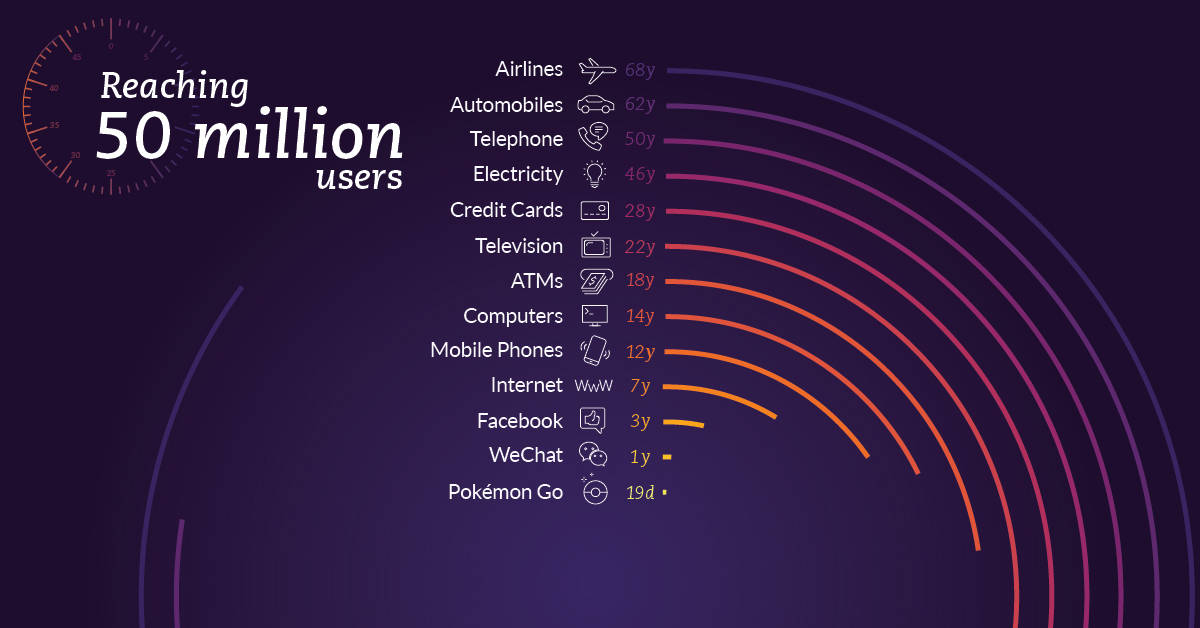
\includegraphics[width=\textwidth]{tech-adoption-time-prev.jpg}
        \caption{How long to reach 50 million users.}
        \label{fig:50milUser}
    \end{figure}

    In the fig.~\ref{fig:50milUser}, from \cite{50milUsers}, is showed how long takes to reach 50 million users, and we can see the very wide difference between car or telephone that required more than 50years and Pokemon Go, only 19 days. So, we can think that before it was reasonable that the copyright cover a product for the entire life of the creator plus 70 years \cite{CopyrightHowLong} because the time to spread that idea require a long time, but nowadays in only 19 days or at most few years that can reach a very vast number of people. So, maybe we can think to reduce this time. But in the other hand we must think that this application that can reach so many person in so few time is also because the owner had a very good idea, in fact this few extraordinary examples are very few.
    
    In my opinion the owner of an idea must have the capability to monetise their idea for a long time, in particular these days that the world is much more competitive rather than few years ago.
    
\section{File Sharing}
    One of the most discussed related topic is File Sharing. Actually file sharing is not illegal, but if you share a copyrighted content it became illegal. One of the most important and pioneer of File Sharing it was The Pirate Bay, main page showed in fig.\ref{fig:piratebay}, that organised and sorted the file, making also some review of that particular content. Before that there was almost only IRC, but too difficult for the majority part of the users and then eMule, user friendly but the majority part of contents were fake and in particular porn.
     \begin{figure}
        \centering
        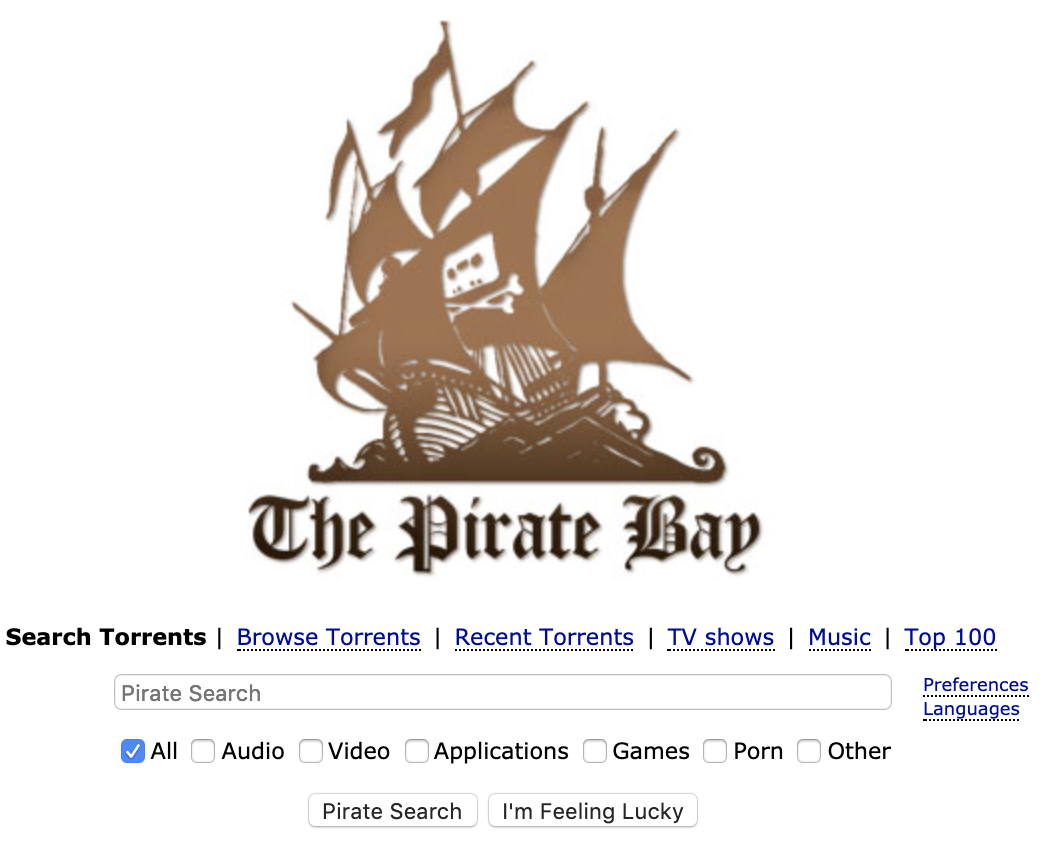
\includegraphics[width=0.5\linewidth]{piratebay.png}
        \caption{This is the homepage of The Pirate Bay in March 2019.}
        \label{fig:piratebay}
    \end{figure}
    
    On this topic we can discuss a lot, in fact if we think that when we buy a book or an audio CD we can decide to lend to our friends and in particular the speaker emphasise the fact that nowadays with new technologies like apple store or play store and in general every service that sell musics or movies or whatever, deny the possibility to lend our goods to our friends.
    
    But in my opinion this involve another concept that is the uniqueness of the products. In particular, it is true that we can lend for example a Book to our friend, but still it is illegal scan our book and make a copy for our friends! So, when we share files we are making numerous copies of that product, so it is not lent a product, but it is copy a product. By the way I think that File Sharing doesn't affect any market furthermore it could improve it. In particular, I believe that a person that really like an artist or a movie will buy that product also if before they have downloaded it, and in addition with the file sharing people have the possibility to know much more content rather than before. The very difference is that now people can judge in advance the work of artists and decide whether they like and they want to buy that product or not.

    Now a question rise spontaneously: why no one stop File Sharing? The reason is quite simple to stop this someone should monitor the network with the consequence that they could see everything illegal document but also legal documents with consequently privacy violation.
    
\section{Governance OF the Internet vs Governance ON the Internet}
    This is a very hot topic, in fact governance of the internet is how internet works, an it is guided by RFC, but Governance on the internet is how governs want guide internet to filter information and manage the news.
    
    In this argument is relevant to mention the Arab Spring where various governments close the access to Internet to their civilian to deny the possibility to connect to social networks and share messages and videos that people could see from around the world. But in this episode the famous group of hackers called Anonymous helped this person that would pronounce their opinion and show what was happening there. In fact, this Group make a DDOS\footnote{DDOS = Distributed Deny of Service} on the government website and at the same time they established some line of communications that allowed the people to leave their messages on tweeter and so on.
    
    This is a citation from the message left from Anonymous "Anonymous can not, and will not stand idly while people are being denied their basic rights and human liberties. ... Anonymous believes this is an outright crime which can not go unpunished.", the entire message is showed in this website \cite{AnonymousEgypt}.
    
    So also this hacker that are usually seen as criminal in some occasions they broke some law in order to reestablish one of the concepts that is at the base of internet and it was expressed by David D. Clark: "We reject: kings, presidents and voting. We believe in: rough consensus and running code"~\cite{DavidC}.
    This concept is strongly related with the concept expressed in the RFC 3271 titled  \textit{The Internet is for Everyone} \cite{Cerf:2002:IE:RFC3271}.
    
\section{Privacy vs Security}
    A strong related topic is how to manage the government security without damage the users' privacy. If fact if you would like to discover the illegal element, as told before, you must track and open every single pack, and this means that you can read the content, damaging in this way the privacy of the sender and receiver.
    Nowadays it is impossible and there are some governments that still monitoring everything. One of the most popular scandal it was about the American government, that was secretly tracking the personal information of everyone, this fact was raised up by Edward Snowden \cite{snowden} a young worker of CIA that denounced this illegal behaviour of his Government. 
    
    People could think that they have nothing to hide and it is not a problem if they are monitored by government, but probably they don't think that their research on Google for example could be misunderstood and for example if a government develop an artificial intelligence able to classify the potential criminal using the research of users... maybe the same person will change their mind and deny the access to their data.
    
    One of the biggest example of this contrast is the TOR\footnote{TOR = The Onion Router} Network \cite{tor}, in fact this project was born to protect the political refugees, and was developed from the federal government of the United States. This software is based on at list three nodes that each has a private key and this guarantee that the source and the receiver are hidden and no one can read the requests and the answer to that.
    But thanks to this security this system is now also called deep web and in particular dark web because this is used as marketing for drugs or weapon, etc.
    
    This is the proof how Privacy and Security is in contradiction.

    

\bibliographystyle{IEEEtran}  
\bibliography{references}

\end{document}
